\documentclass{article}
\usepackage[utf8]{inputenc}
\usepackage[spanish]{babel}\decimalpoint
\usepackage{graphicx}
\graphicspath{ {Imagenes/} }
\usepackage{float}
\usepackage{minted}

\title{
\includegraphics[scale=.15]{LogoTec.png}\\Reporte final del reto}


\author{ Francisco Leonid Gálvez Flores, A01174385\and
Isaac Arredondo Padrón, A00828359\and
Miguel Ángel Chávez Robles, A01620402\and
Salette Guadalupe Noemi Villalobos, A01246619}
\begin{document}
\renewcommand{\baselinestretch}{1.5}


\maketitle


\pagebreak

\tableofcontents

\pagebreak


\section{Conocimiento del negocio}

\subsection{Objetivos del Negocio}

CEMEX busca reducir el gasto de energía manteniendo un nivel mínimo de calidad. Para esto, tienen en producción una combinación de maquinaria eléctrica y combustible, las máquinas eléctricas entregan un nivel de calidad superior, mientras que las de energía combustible son más baratas de operar. Además de la tasa de producción, se debe considerar la dureza del acero utilizado tanto para el gasto eléctrico como para la calidad del producto esperado.

\subsection{Situación actual del Negocio}

Actualmente están en busca de una combinación de energías eléctrica y calorífica que les permitan alcanzar los objetivos previamente planteados, por lo que están realizando pruebas y solicitando el apoyo a estudiantes de ingeniería en ciencia de datos y matemáticas. \cite{reto}

\subsection{Objetivos a nivel de minería de datos}\label{objetivos}
\begin{itemize}
    \item Optimizar el uso de energía eléctrica y fósil de la planta de producción de acero de CEMEX.
    \item Buscar correlaciones entre las variables disponibles
    \item Comprender cómo interactúan las variables entre ellas
    \item Crear un modelo que dadas x variables de entrada brinde como salida el uso óptimo de energía 
    \item Minimizar el uso de energía eléctrica, pues es la que es más cara para la empresa, pero usar estas máquinas entrega una mejor calidad respecto a las de combustible fósil
\end{itemize}

\subsection{Plan del proyecto}
El plan del proyecto dependerá de cinco etapas claves, las cuales se definen a continuación:
\begin{enumerate}
    \item Extracción de datos(Semana 1):
    \subitem Esta etapa se enfoca en la importación de datos
    
    \item Exploración de datos(Semana 2):
    \subitem Estudiar las variables, definir cuales son importantes para el objetivo y cuáles no
    \subitem Explorar el dataframe, definir puntos de gestión de calidad de los datos
    
     \item Preprocesamiento de datos(Semana 3):
    \subitem Hacer eliminación de variables innecesarias y/o redundantes
    \subitem Eliminar datos con registros nulos
    \subitem Hacer eliminación de datos atípicos para no contar con anomalías en los datos
    \subitem Modificar el índice de la fecha, de manera que este sea un objeto date en lugar de un objeto genérico de Pandas
    
    \item Modelación(Semana 4 y 5):
    \subitem Determinar cuáles serán las variables de las cuales generamos predicciones así como cuales usar para predecir estas.
    \subitem Determinar el conjunto de datos que optimizaran la energía para cada valor de las variables de producción
    \subitem Dividir el conjunto de datos anterior en subconjuntos de entrenamiento y de evaluación  
    \subitem Crear 2 modelos de regresión
    \subitem Entrenar los conjuntos de regresión
    
    \item Evaluación y creación de una aplicación web(Semana 5):
    \subitem Evaluar los modelos creados usando métodos de cross validation, determinar cual modelo entrega mejores resultados, asegurándose de que cada uno de estos modelos esté funcionando con los parámetros óptimos, evitando el overfitting


\end{enumerate}




\subsection{Antecedentes del negocio}

CEMEX es una empresa líder global en su campo, la venta de cemento y productos industriales similares. Fundada en 1906 en la ciudad de Hidalgo, Nuevo León, ha crecido hasta rebasar los 40,000 empleados, y ha expandido sus operaciones a múltiples lugares, teniendo más de 250 plantas de concreto y 95 centros de distribución. \cite{cemex}. 

Dentro de los múltiples desafíos que una empresa de este calibre encuentra, está la optimización de recursos energéticos. Para lograr este fin han llevado registro de distintas variables que describen este proceso, tales como 
Buscan reducir el gasto energético al procesar acero, esto deben hacerlo logrando una relación óptima entre máquinas que usan energía combustible y energía eléctrica. Se sabe que la energía combustible le cuesta $0.724$ veces a la empresa lo que la energía eléctrica, pero las máquinas que usan energía eléctrica entregan un trabajo de mayor calidad. \cite{reto} 

\section{Comprensión de los datos}


\subsection{Procesos de captura de datos}


Los datos de la base de datos se recabaron desde el $1^{ro}$ de enero del año 1995 hasta el 30 de diciembre del año 2019, normalmente con entradas diarias en las cuales incluían: La fecha, dureza, tasa de producción, consumo de energía eléctrica, consumo de energía calórica, etc.

Para poder manipular los datos usamos la base de datos en formato CSV, así como la librería Pandas, esta sirve para manipular conjuntos de datos de una manera muy eficiente, permite operaciones de creación, lectura, modificación, eliminación, búsqueda, conteo, etc. \cite{reback2020pandas}


\subsection{Descripción de los datos}

\begin{figure}[ht]
\hfill
\begin{tabular}{|c|c|c|c|c|c|}
\hline
Q & Time & D & Tasa\_Prod\\
\hline
Calidad &
Timestamp &
Dureza del acero &
Tasa de producción \\
\hline
\end{tabular}

\begin{tabular}{|c|c|c|}
    \hline
     EC & EE &Asp  \\
     \hline
Energía combustible &
Energía eléctrica &
Se desconoce el contexto de la variable\\
\hline
\end{tabular}


\caption{Tabla 1. Se describen las variables que representan nuestros registros de datos.[Creación propia, 2021]}
\label{Tabla 1}
\end{figure}

\begin{itemize}
    \item El campo de calidad es un valor normalizado que se encuentra entre 0 y 1
    \item El campo time es una estampa de tiempo del momento en el que se capturaron los datos
    \item El campo D nos dice la dureza del acero usado, sus valores van de 80 a 112
    \item El campo Tasa\_Prod indica la tasa de producción necesaria, sus valores van de 0 a 480
    \item No se conoce que representa la variable Asp
\end{itemize}


\subsection{Exploración de los datos}\label{edd}
Al momento de importar los datos, se observan 9389 entradas, de las cuales solo existe un dato nulo, el cual se encuentra en la columna de dureza. Todos los datos que se espera que sean numéricos lo son, no es necesario convertirlos, la única columna que requiere un cambio es la de Time, podemos convertir este campo a date-time sin problema. Lo anterior nos refleja que los datos tienen bastante calidad y facilita la limpieza de los mismos. 



\subsection{Gestión de la calidad de datos}\label{cdd}

Los datos parecen encontrarse en buen estado. Para tener un conjunto de datos de calidad solo es necesario: transformar el campo Time a su formato correcto, se elimina el campo Asp y se eliminan los registros con valores nulos, además de la normalización de datos eliminando valores atípicos. Estas tareas son parte de la sección \ref{ldd}.



\subsection{Artículos relacionados con el tema}

\subsubsection{Optimización aplicada a sistemas de bombeo}

Sabogal Abril, B. R. , Palacios Peñaranda, J. A., \& Pantoja Tovar, C. L. realizaron un proyecto similar para optimizar el uso de energía eléctrica en sistemas de bombeo, en este analizaron el impacto de usar frecuencias distintas con el objetivo de encontrar un modelo que les permitiera disminuir el uso de energía eléctrica. Tras recolectar una variedad de datos en distintas observaciones concluyeron que era posible un ahorro operando en un punto óptimo reduciendo la potencia necesaria mediante variaciones de velocidad. \cite{oesb}

\subsubsection{Estimación de potencial fotovoltaico }
En cuatro ciudades de Colombia utilizan la información recopilada en Bogotá, Cúcuta, Manizales y Pasto para con el empleo del software MATLAB se sometan los datos a dos algoritmos de comparación : K-means y Fuzzy C-means y uno de visualización: Análisis de componentes principales (PCA) todo esto con el fin de determinar la factibilidad de la implementación de las micro-redes. \cite{torres2019estimacion}


\subsubsection{Predicción de costos de PYMES}
Un algoritmo se encarga de predecir los costos del consumo eléctrico de las micro, pequeñas y medianas empresas del sector de alimentos. Utilizando el perfil de consumo y tarifa eléctrica para reproducir los gastos y escenarios del cambio de tarifa. De esta forma, se facilitó reconocer la tarifa más eficiente para cada una de las empresas considerando además la retroalimentación del usuario. Este es un ejemplo de cómo la metodología lleva a la productividad y competitividad de las empresas.\cite{cuisano2020eficiencia}

\subsubsection{Optimización de recursos hídricos}

En el artículo se especifica que la Provincia de Mendoza emplea herramientas digitales para optimizar el uso del agua proyectando además, con la utilización de una máquina de Inteligencia Artificial, el impacto económico que provoca esta acción en su matriz productiva. \cite{inproceedings}

\subsubsection{Agricultura de precisión}

Expone la propuesta de una red de sensores que es capaz de optimizar una plantación de café a través de una red sensorial con distintos nodos comunicados entre si usados para conocer los estados de temperatura, humedad, y radiación solar, y otras características de los cultivos, de esta manera se cuida el uso de recursos en la plantación teniendo información más profunda sobre su estado actual, ayudando a reducir costos. \cite{urbano2013redes}

\section{Preparación de los datos}
\subsection{Establecer el universo de datos con los que trabajar}

Como se mencionó en la sección \ref{cdd}, la única variable que debe ser eliminada es la de Asp, el resto de campos son útiles para el objetivo. En cuanto a los datos atípicos, se considerarán atípicos todos los datos que estén alejados más de 2 desviaciones estándar de la media. 

\subsection{Limpieza de datos}\label{ldd}
\begin{itemize}
    \item Para eliminar los campos innecesarios usamos la función drop
    \item Para limpiar los datos vacíos se usa la función dropna 
    \item Para limpiar los datos atípico se usa la función Zscore de la librería Scipy \cite{2020SciPy-NMeth}, para calcular el valor z de cada entrada por separado, y eliminar los valores cuyo valor z sea mayor a 2. Al usar la prueba Z, se están normalizando los datos sin necesidad de cambiar sus magnitudes
\end{itemize}

\begin{minted}{python}
import pandas as pd
import scipy as sp 
df=df.drop('Asp', axis = 1)
df.dropna()
sp.stats.zscore(df.<campo>))
\end{minted}



\subsection{Construir un juego de datos apto para ser usado para la modelación}\label{construir}

Se busca determinar si existen correlaciones entre los datos, para esto se usa una matriz de correlaciones, la cual devuelve el coeficiente de correlación de Pearson de cada variable con otra. Usando un heatmap obtenemos una representación mas visual de estas correlaciones. En el libro \emph{Handbook of Biological Statatistics} se menciona que este coeficiente funciona bien con variables que siguen una distribución normal, pero aún así es tan robusto que no se ve afectado en gran medida si hay perdida de normalidad\cite{mcdonald2009handbook}.  

\begin{figure}[h!]
    \centering
    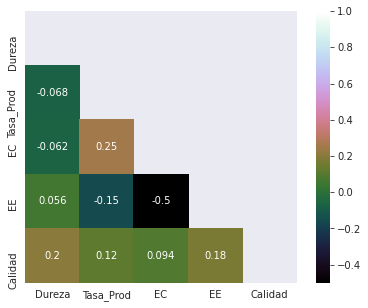
\includegraphics[scale=.7]{histogramas/img8.png}
    \caption{Heatmap de matriz de correlaciones con diagonal principal y simetría suprimida [Creación propia, 2021]}
    \label{fig:heatmap}
\end{figure}

\pagebreak
La distribución que siguen las variables es la siguiente:

\begin{figure}[H]
    \centering
    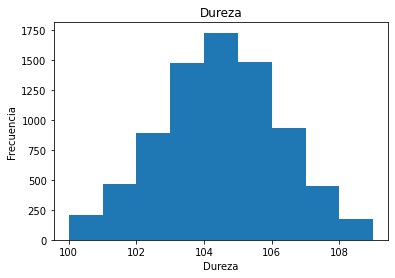
\includegraphics[scale=.7]{histogramas/img3.png}
    \caption{Distribución de valores de dureza [Creación propia, 2021]}
    \label{fig:dureza}
\end{figure}

\begin{figure}[H]
    \centering
    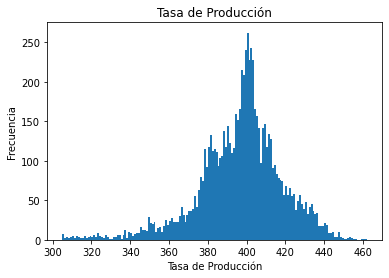
\includegraphics[scale=.7]{histogramas/img4.png}
    \caption{Distribución de valores de tasa de producción [Creación propia, 2021]}
    \label{fig:tasa}
\end{figure}

\begin{figure}[H]
    \centering
    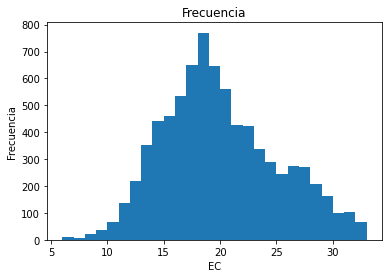
\includegraphics[scale=.7]{histogramas/img5.png}
    \caption{Distribución de valores de energía combustible [Creación propia, 2021]}
    \label{fig:ee}
\end{figure}

\begin{figure}[H]
    \centering
    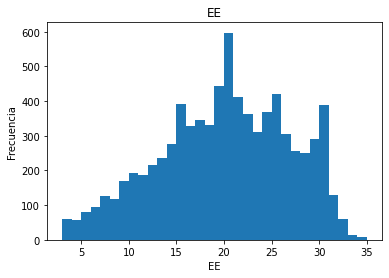
\includegraphics[scale=.7]{histogramas/img6.png}
    \caption{Distribución de valores de energía eléctrica [Creación propia, 2021]}
    \label{fig:ec}
\end{figure}

\begin{figure}[H]
    \centering
    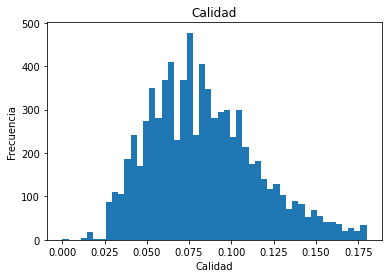
\includegraphics[scale=.7]{histogramas/img7.png}
    \caption{Distribución de valores de calidad [Creación propia, 2021]}
    \label{fig:calidad}
\end{figure}


Tras ver las distribuciones podemos argumentar que, aunque no es un ajuste perfecto, las variables sí se asemejan a una distribución normal, por lo que podemos confiar en la robustez de el coeficiente de correlación. 


\begin{figure}[H]
    \centering
    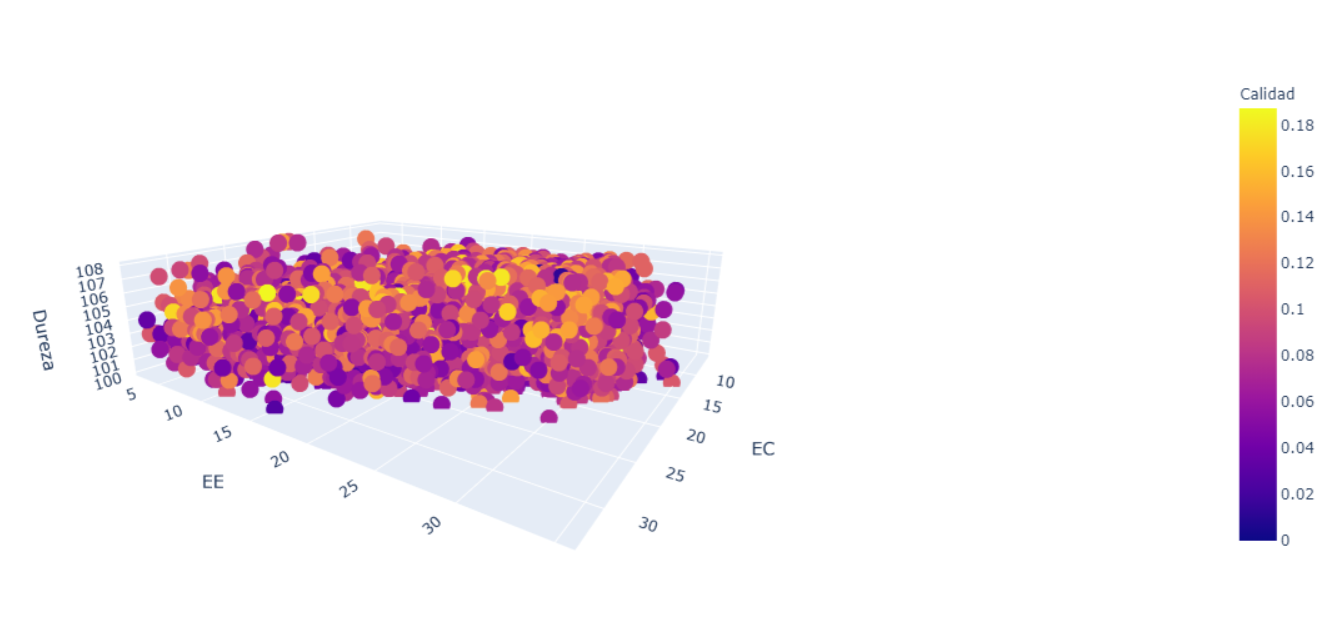
\includegraphics[scale=.5]{img9.png}
    \caption{Dispersión EE, EC, Dureza [Creación propia, 2021]}
    \label{fig:3d}
\end{figure}



En este punto se cuenta con un buen dataset en cuestión de calidad de datos, sin embargo, no está listo para cumplir el propósito de optimizar el gasto energético. Para tener una idea de que datos son aptos para esto  se calcula el costo y uso ponderado de la energía. Este costo se obtiene de la siguiente manera:


\begin{equation}\label{eq1}
    CostoPonderado_{i}=\frac{(EC_{i})(0.724)+EE_{i}}{Tasa\_prod_{i}}
\end{equation}
Donde $i$ es la $i$esima entrada. 

\begin{equation}
    EEPonderdo_{i}=\frac{EE_{i}}{Tasa\_prod_{i}}
\end{equation}
Donde $i$ es la $i$esima entrada. 


\begin{equation}
    ECPonderdo_{i}=\frac{EC_{i}}{Tasa\_prod_{i}}
\end{equation}
Donde $i$ es la $i$esima entrada. 


Una vez que se han obtenido los costos ponderados usando la ecuación \ref{eq1}, definimos el conjunto de datos final usando las entradas cuyo costo ponderado es menor o igual a 0.075. De esta manera el modelo será construido con los datos que tienen una relación mejor entre costo y tasa de producción en términos monetarios.

Los datos de entrenamiento y prueba se obtuvieron usando la función train\_test\_split de la librería Sklearn \cite{scikit-learn}. 
Se usó la relación estándar 80\% datos de entrenamiento y 20\% datos de prueba. Al momento de separar los datos también se eliminó la columna de TIME pues es irrelevante para el modelado.

\section{Modelación y evaluación de datos}

\subsection{Seleccionar las técnicas de modelado más adecuadas para nuestro juego de datos y nuestros objetivos}\label{tecnicas}

Derivado a la naturaleza de las predicciones,  se espera obtener como resultado un modelo con múltiples salidas. Por ello, se eligieron los modelos de K-Nearest Neighbors y Linear Regression con Multi-Output.
Para K-Nearest Neighbors se consideraron sus principales ventajas:
\begin{itemize}
    \item No asume información sobre los datos.
    
    En la mayoría de los modelos se hacen suposiciones sobre los datos y sobre el tipo de distribución que estos llevan, sin embargo KNN evita este inconveniente.\cite{BonnerL2018}
    \item Se entrena en el momento de la predicción.
    
    KNN crea las clases que van a determinar la predicción simultáneamente al realizar esta, gracias a ello se pueden afectar nuevos datos sin que creen un desbalance.\cite{BonnerL2018}
    \item Fácil implementación para multivariables.
    
    Esto representa una ventaja pues el modelo va a tener tres variables de entrada.
    \cite{BonnerL2018} 
\end{itemize}

Por su parte, la regresión lineal fue elegida para comparar los comportamientos de las predicciones utilizando un modelo lineal y un no-lineal.

\subsection{Fijar una estrategia de verificación de la calidad del modelo}
La primera métrica que se empleará es $R^{2}_{ajustada}$.Según el libro \emph{Handbook of Applied Muiltivariate Statistics and Mathematical Modeling}, esta es una métrica que permite evaluar fácilmente distintos modelos de regresión que cuentan con un número distinto de estimadores. A diferencia de la $R^2$ simple, $R^{2}_{ajustada}$ agrega una penalización por cada estimador usado, este parte de la idea de que usar más estimadores no necesariamente es mejor \cite{handbook}, es por esto que, en nuestro caso, probablemente $R^{2}_{ajustada}$ sea bajo, pero eso no convierte al modelo en inservible. En la Figura \ref{fig:R2Ajustada} se observan sus componentes:
\begin{figure}[h!]
    \centering
    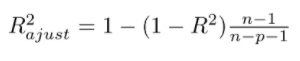
\includegraphics[scale=.7]{F4/F4-RAjustada.PNG}
    \caption{Fórmula de $R^{2}_{ajustada}$.\cite{RajustadaCita}}
    \label{fig:R2Ajustada}
\end{figure}

La segunda métrica por usar será el Error Absoluto Medio, en el libro \emph{Machine Learning for Developers} se menciona que la métrica \emph{Mean absolute error}, computa el error medio absoluto, que corresponde a el valor esperado de la perdida del error, es decir, cuanto se espera que el modelo se equivoque en cada predicción \cite{mlfd}. En la Figura \ref{fig:MAE} se observan los componentes:

\begin{figure}[h!]
    \centering
    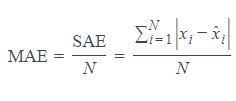
\includegraphics[scale=.7]{F4/F4-MAE.PNG}
    \caption{Fórmula de Error Absoluto Medio.\cite{MAECita}}
    \label{fig:MAE}
\end{figure}

\subsection{Construir un modelo a partir de la aplicación de las técnicas seleccionadas sobre el juego de datos}\label{apto}

Primero se se separaron los datos en aquellos que servirían para la optimización, con este propósito se construyó una gráfica comparativa entre la Calidad y el Costo Ponderado. Se puede observar en la Figura \ref{fig:costo_calidad}

\begin{figure}[h!]
    \centering
    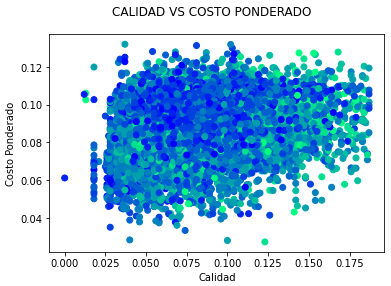
\includegraphics[scale=.7]{F4/F4-im1.PNG}
    \caption{Representación de la relación entre costo ponderado y calidad. Distribución semejante a la normal con concentración de los datos en el centro.[Creación propia, 2021]}
    \label{fig:costo_calidad}
\end{figure}


Tomando en cuenta la limpieza de calidad que se generó en los pasos anteriores, los puntos que se encuentran aquí cumplen con la calidad que se espera del modelo, derivado de esto, hace falta limitar el costo ponderado para así obtener los puntos óptimos para ello se seleccionaran tres cotas superiores para el costo ponderado formando tres subconjuntos de datos sobre los cuales aplicar los modelos.

\subsubsection{Primer Conjunto de Datos}

El primer grupo de variables que se formará será tomando como cota superior el valor de Costo Ponderado  a 0.075. Es decir, elegiremos aquellos datos con un precio menor o igual a 0.075. Los datos se observan en la Figura \ref{fig:costo_calidad_acotada1}:
\pagebreak
\begin{figure}[!h]
    \centering
    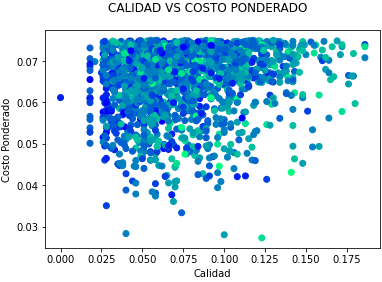
\includegraphics[scale=.7]{F4/F4-im2.PNG}
    \caption{Datos que cumplen con las características de calidad con un costo menor o igual 0.075. [Creación propia].}
    \label{fig:costo_calidad_acotada1}
\end{figure}

Se eligió ese umbral ya que logra mantener un costo bajo, uno de nuestros objetivo, sin limitar excesivamente la cantidad de los datos evitando así el peligroso Overfitting.

Después de determinar el conjunto de datos sobre el que se trabajará, se procedió a repararlos en subconjuntos de entrenamiento (training) y prueba (test). Los valores que se utilizaron fueron 80\% y 20\%, así se aseguró una cantidad considerable para realizar el ajuste del modelo. Además, se seleccionaron aleatoriamente, con el fin de mantener una independencia entre los datos. Esta será también la manera en la que separaremos los siguiente dos subconjuntos.

Primero se aplicó el modelo K Nearest Neighbors. Se comenzó por seleccionar un K adecuada para el modelo. El valor K representa el número de valores cercanos que se eligen para determinar el promedio que al final será el valor asignado a la variable siendo predicha. El valor K óptimo depende de cada regresión, en general se utiliza aquel que comienza a dar un Error Medio Cuadrático Estable. Se advierte que al elegir un valor K bajo se puede caer en el Overfitting, en caso contrario al utilizar un valor K alto la modelación puede ser más acertada pero los valores en los extremos están muy indeterminados.\cite{Mille2019} 

\begin{figure}[!h]
    \centering
    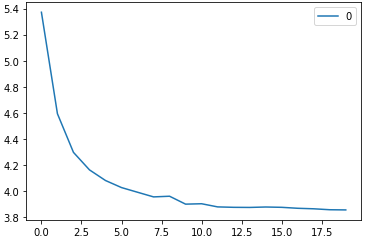
\includegraphics[scale=.7]{F4/F4-im3.PNG}
    \caption{Error Cuadrático Medio, gráfica para identificar el valor óptimo de K. [Creación propia, 2021]}
    \label{fig:Codo1}
\end{figure}

Implementamos el valor K=12 pues es en ese momento cuando la curva en la Figura \ref{fig:Codo1} comienza a volverse constante, además consideramos que es un número apropiado para evitar el Overfitting tomando en cuenta la cantidad de datos que tenemos.
\pagebreak

Al aplicar el modelo podemos obtener algunas predicciones como las de la Figura \ref{fig:Prediccion1.1}: 

\begin{figure}[!h]
    \centering
    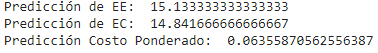
\includegraphics[scale=.7]{F4/F4-im4.PNG}
    \caption{Predicciones creadas por el modelo de KNN en el primer conjunto de datos.[Creación propia, 2021]}
    \label{fig:Prediccion1.1}
\end{figure}

Y las gráficas que comparan los valores de los valor de Energía Eléctrica, Energía Combustible y Costo Ponderado predichos (de prueba) y los reales son: 

\begin{figure}[!h]
    \centering
    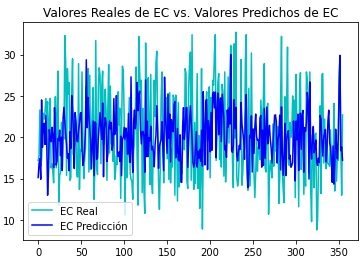
\includegraphics[scale=.7]{F4/F4-im5.PNG}
    \caption{Comparación de los valores de EC vs. los predichos. Modelo KNN primer conjuntos de datos.[Creación propia, 2021]}
    \label{fig:EC1.1}
\end{figure}

\begin{figure}[!h]
    \centering
    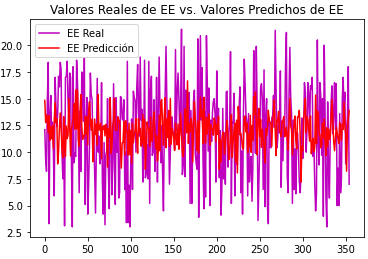
\includegraphics[scale=.7]{F4/F4-im6.PNG}
    \caption{Comparación de los valores de EE vs. los predichos. Modelo KNN primer conjunto de datos.[Creación propia, 2021]}
    \label{fig:EE1.1}
\end{figure}

\begin{figure}[!h]
    \centering
    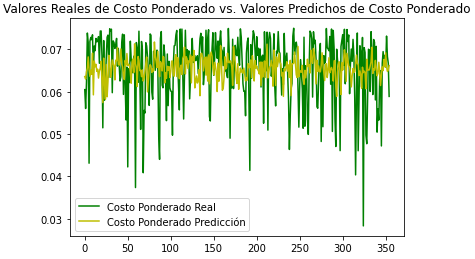
\includegraphics[scale=.7]{F4/F4-im7.PNG}
    \caption{Comparación de los valores de Costo Ponderado vs. los predichos. Modelo KNN primer conjunto de datos.[Creación propia, 2021]}
    \label{fig:CostoPonderado1.1}
\end{figure}

En las Figuras \ref{fig:EC1.1}, \ref{fig:EE1.1} y \ref{fig:CostoPonderado1.1} se busca observar que las variables realmente tengan un comportamiento semejante al de las originales, pues aunque no sean iguales los valores de lo real y lo predicho, mientras se comporten similarmente la predicción puede ser muy buena o aceptable. Como se puede observar en las figuras anteriores, los valores sí siguen un mismo patrón de comportamiento. Los ascensos y descensos tienen una ubicación similar para las gráficas de los valores reales y los predichos. 

El segundo regresor será Multi Output Regressor con la Regresión Lineal. Se utiliza la librería Multi Output para obtener diversas variables de salida, sin embargo el concepto sigue siendo igual al de una Regresión Lineal Multivariada, donde en general se busca minimizar el error cuadrado.

Su aplicación es más sencilla pues únicamente se debe entrenar el modelo con los subconjuntos de entrenamiento ya anteriormente seleccionados. Un ejemplo de las predicciones realizadas por el modelo son: 

\begin{figure}[!h]
    \centering
    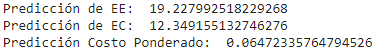
\includegraphics[scale=.7]{F4/F4-im8.PNG}
    \caption{Predicciones creadas por el modelo de Regresión Lineal en el primer conjunto de datos.[Creación propia, 2021]}
    \label{fig:predicciones1.2}
\end{figure}

Como se puede observar en la Figura \ref{fig:predicciones1.2} , no tiene mucho sentido que el Costo Ponderado sea tan bajo, apenas un poco más alto que el de KNN, mientras que la energía EE, aquella que implica un mayor gato, es tan elevada. Por ello podemos cuestionar la validez del modelo. 

Las gráficas que comparan los valores reales y predichos son: 
\begin{figure}[!h]
    \centering
    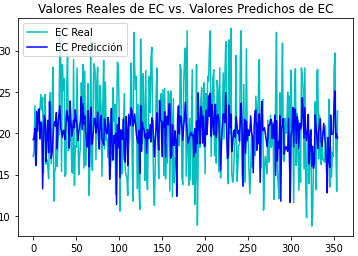
\includegraphics[scale=.7]{F4/F4-im9.PNG}
    \caption{Comparación de los valores de EC vs. los predichos. Modelo Regresión Lineal primer conjunto de datos.[Creación propia, 2021]}
    \label{fig:EC1.2}
\end{figure}

\begin{figure}[!h]
    \centering
    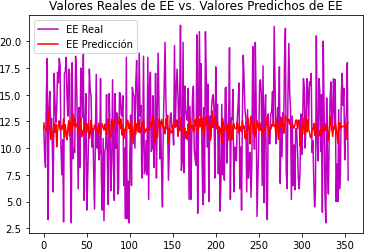
\includegraphics[scale=.7]{F4/F4-im10.PNG}
    \caption{Comparación de los valores de EE vs. los predichos. Modelo Regresión Lineal primer conjunto de datos.[Creación propia, 2021]}
    \label{fig:EE1.2}
\end{figure}

\begin{figure}[!h]
    \centering
    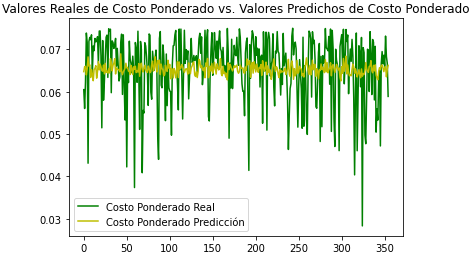
\includegraphics[scale=.7]{F4/F4-im11.PNG}
    \caption{Comparación de los valores de Costo Ponderado vs. los predichos. Modelo Regresión Lineal primer conjunto de datos.[Creación propia, 2021]}
    \label{fig:CostoPonderado1.2}
\end{figure}
\pagebreak
Como se puede observar las Figuras \ref{fig:EC1.2}, \ref{fig:EE1.2} y \ref{fig:EE1.2}, aunque siguen un cierto patrón similar, lo cierto es que los valores predichos tienen un mayor número de depresiones que no suceden en los datos originales, de esta manera se determina que el modelo no sigue el mismo comportamiento de los datos originales.

\subsubsection{Segundo Conjunto de Datos} 
En este caso tomamos un precio máximo de 0.06, como se observa en la Figura \ref{fig:costo_calidad_acotada2} esto puede limitar notablemente nuestra cantidad de datos, pero también representa una disminución buscada en el precio.

\begin{figure}[!h]
    \centering
    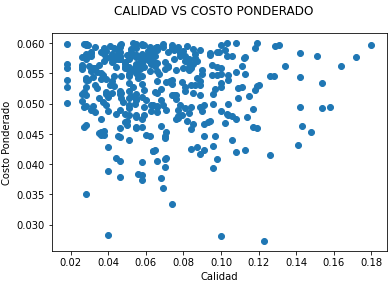
\includegraphics[scale=.7]{F4/F4-im12.PNG}
    \caption{Datos que cumplen con las características de calidad con un costo menor o igual 0.06. [Creación propia]. }
    \label{fig:costo_calidad_acotada2}
\end{figure}\pagebreak

Para aplicar el modelo K Nearest Neighbors se mantuvo el mismo procedimiento descrito anteriormente:

\begin{figure}[!h]
    \centering
    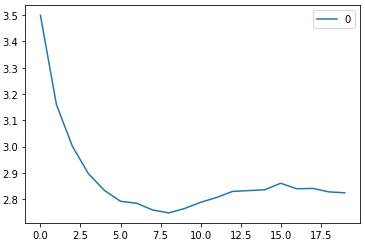
\includegraphics[scale=.7]{F4/F4-im13.PNG}
    \caption{Error Cuadrático Medio, gráfica para identificar el valor óptimo de K. [Creación propia, 2021]}
    \label{fig:Codo2}
\end{figure}

Se conserva la K=12 porque también en este caso es cuando la gráfica comienza a tomar valores constantes (Figura \ref{fig:Codo2}). 

Se aplica el modelo y se obtienen los siguientes resultados:
\begin{figure}[!h]
    \centering
    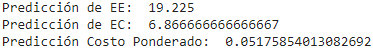
\includegraphics[scale=.7]{F4/F4-im14.PNG}
    \caption{Predicciones creadas por el modelo de KNN en el segundo conjunto de datos.[Creación propia, 2021]}
    \label{fig:Prediccion2.2}
\end{figure}

Como se puede observar en la Figura \ref{fig:Prediccion2.2} la combinación es mucho menos fiable que la del modelo anterior pues al tener una Energía Eléctrica tan elevada, es poco probable tener un Costo Ponderado tan bajo como 0.05.
\pagebreak

Las gráficas que nos ayudan a visualizar el comportamiento del modelo son:
\begin{figure}[!h]
    \centering
    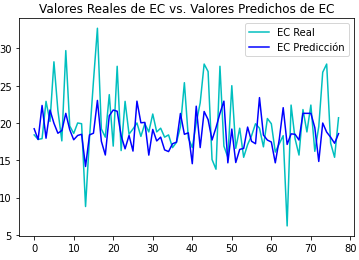
\includegraphics[scale=.7]{F4/F4-im15.PNG}
    \caption{Comparación de los valores de EC vs. los predichos. Modelo  KNN el segundo conjunto de datos.[Creación propia, 2021]}
    \label{fig:EC2.1}
\end{figure}

\begin{figure}[!h]
    \centering
    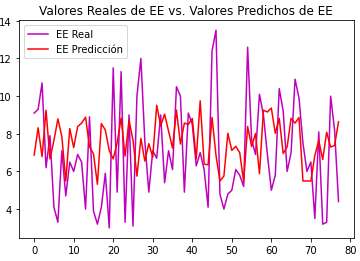
\includegraphics[scale=.7]{F4/F4-im16.PNG}
    \caption{Comparación de los valores de EE vs. los predichos. Modelo KNN segundo conjunto de datos.[Creación propia, 2021]}
    \label{fig:EE2.1}
\end{figure}

\begin{figure}[!h]
    \centering
    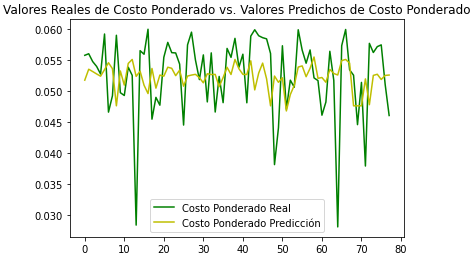
\includegraphics[scale=.7]{F4/F4-im17.PNG}
    \caption{Comparación de los valores de Costo Ponderado vs. los predichos. Modelo KNN segundo conjunto de datos.[Creación propia, 2021]}
    \label{fig:CostoPonderado2.1}
\end{figure}
\pagebreak
Se observa en las Figuras \ref{fig:EC2.1}, \ref{fig:EE2.1} y \ref{fig:CostoPonderado2.1} que en este caso los datos siguen un patrón similar al de los datos originales, sin embargo, el modelo de KNN con el primer conjunto de datos continúa manteniendo un comportamiento todavía más similar.


Se procede con el modelo de regresión lineal que arroja las predicciones (Figura \ref{fig:predicciones2.2}): 
\begin{figure}[!h]
    \centering
    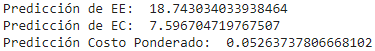
\includegraphics[scale=.7]{F4/F4-im18.PNG}
    \caption{Predicciones creadas por el modelo de Regresión Lineal en el segundo conjunto de datos.[Creación propia, 2021]}
    \label{fig:predicciones2.2}
\end{figure}


Los resultados son muy semejantes a los del modelo aplicado en el primer conjunto de datos, lo que indica que no es un modelo muy confiable. 

Para analizar su comportamiento se presentan las Figuras \ref{fig:EC2.2}, \ref{fig:EE2.2} y \ref{fig:CostoPonderado2.2} : \pagebreak

\begin{figure}[!h]
    \centering
    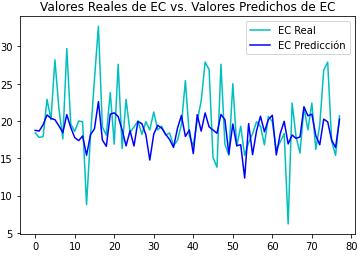
\includegraphics[scale=.7]{F4/F4-im19.PNG}
    \caption{Comparación de los valores de EC vs. los predichos. Modelo Regresión Lineal segundo conjuntos de datos.[Creación propia, 2021]}
    \label{fig:EC2.2}
\end{figure}

\begin{figure}[!h]
    \centering
    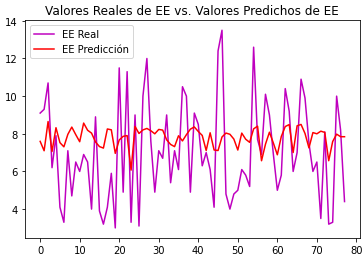
\includegraphics[scale=.7]{F4/F4-im20.PNG}
    \caption{Comparación de los valores de EE vs. los predichos. Modelo Regresión Lineal segundo conjunto de datos.[Creación propia, 2021]}
    \label{fig:EE2.2}
\end{figure}

\begin{figure}[!h]
    \centering
    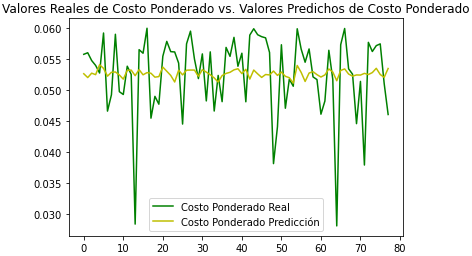
\includegraphics[scale=.7]{F4/F4-im21.PNG}
    \caption{Comparación de los valores de Costo Ponderado vs. los predichos. Modelo Regresión Lineal segundo conjunto de datos.[Creación propia, 2021]}
    \label{fig:CostoPonderado2.2}
\end{figure}
\pagebreak
El patrón de comportamiento es todavía más inexacto pues este sigue una línea casi horizontal cuando el modelo original se compone por muchas crestas y depresiones.

\subsubsection{Tercer Conjunto de Datos}

Se redujo incluso más el grupo de datos, de forma que se logre ser más estrictos con la reducción de costos, sin embargo al mantener un conjunto tan pequeño, es mucho el riesgo de que el algoritmo no tenga suficiente capacidad para aprender correctamente los patrones. 

El umbral que se utilizó fue de 0.055, como se observa en la Figura \ref{fig:costo_calidad_acotada3}:

\begin{figure}[!h]
    \centering
    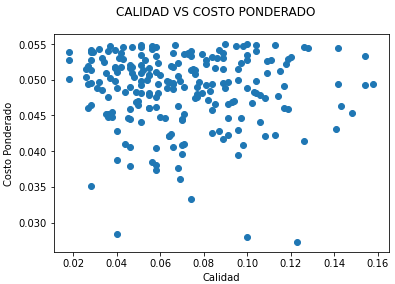
\includegraphics[scale=.7]{F4/F4-im22.PNG}
    \caption{Datos que cumplen con las características de calidad con un costo menor o igual 0.055. [Creación propia].}
    \label{fig:costo_calidad_acotada3}
\end{figure}
\pagebreak

Para aplicar KNN se busca la K:

\begin{figure}[!h]
    \centering
    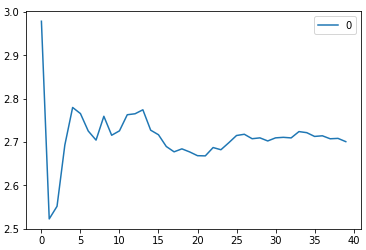
\includegraphics[scale=.7]{F4/F4-im23.PNG}
    \caption{Error Cuadrático Medio, gráfica para identificar el valor óptimo de K. [Creación propia, 2021]}
    \label{fig:Codo3}
\end{figure}

Se observa en la Figura \ref{fig:Codo3} un comportamiento errático que dificulta la identificación del punto constante. Sin embargo, de acuerdo con nuestro criterio, el punto óptimo es K=20, pues la gráfica deja de tener cambios tan bruscos. 

\begin{figure}[!h]
    \centering
    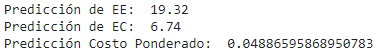
\includegraphics[scale=.7]{F4/F4-im24.PNG}
    \caption{Predicciones creadas por el modelo de KNN en el tercer conjunto de datos.[Creación propia, 2021]}
    \label{fig:Prediccion3.1}
\end{figure}

Los valores predichos en la Figura \ref{fig:Prediccion3.1} son todavía más improbables pues implican un nivel igual de elevado de la Energía Eléctrica con un Costo Ponderado mucho más bajo. \pagebreak

\begin{figure}[!h]
    \centering
    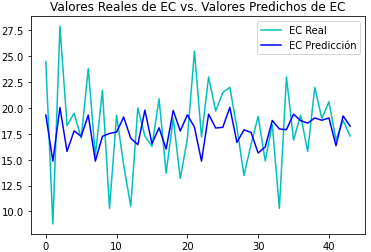
\includegraphics[scale=.7]{F4/F4-im25.PNG}
    \caption{Comparación de los valores de EC vs. los predichos. Modelo  KNN el tercer conjuntos de datos.[Creación propia, 2021]}
    \label{fig:EC3.1}
\end{figure}

\begin{figure}[!h]
    \centering
    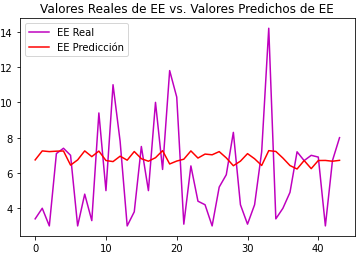
\includegraphics[scale=.7]{F4/F4-im26.PNG}
    \caption{Comparación de los valores de EE vs. los predichos. Modelo KNN tercer conjunto de datos.[Creación propia, 2021]}
    \label{fig:EE3.1}
\end{figure}

\begin{figure}[!h]
    \centering
    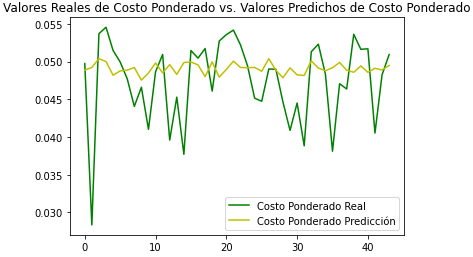
\includegraphics[scale=.7]{F4/F4-im27.PNG}
    \caption{Comparación de los valores de Costo Ponderado vs. los predichos. Modelo KNN tercer conjunto de datos.[Creación propia, 2021]}
    \label{fig:CostoPonderado3.1}
\end{figure}
\pagebreak
Mientras que la Figura \ref{fig:EC3.1} asemeja ligeramente el comportamiento, el resto de las Figuras \ref{fig:EE3.1} y \ref{fig:CostoPonderado3.1} distan mucho de tener unos valores predichos comparables con los valores reales.

En cuanto al modelo de Regresión Lineal, los valores obtenidos son (Figura \ref{fig:predicciones3.2}):

\begin{figure}[!h]
    \centering
    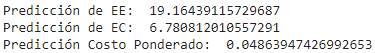
\includegraphics[scale=.7]{F4/F4-im28.PNG}
    \caption{Predicciones creadas por el modelo de Regresión Lineal en el tercer conjunto de datos.[Creación propia, 2021]}
    \label{fig:predicciones3.2}
\end{figure}

Semejantes a los del modelo anterior, no tienen sentido por la misma razón de lo poco probable que es obtener un Costo Ponderado tan pequeño con ese uso de Energía Eléctrica.

Sus gráficas son las Figuras \ref{fig:EC3.2}, \ref{fig:EE3.2} y \ref{fig:CostoPonderado3.2}: \pagebreak

\begin{figure}[!h]
    \centering
    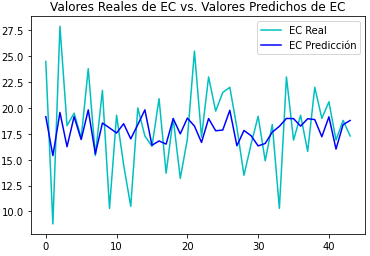
\includegraphics[scale=.7]{F4/F4-im29.PNG}
    \caption{Comparación de los valores de EC vs. los predichos. Modelo Regresión Lineal tercer conjuntos de datos.[Creación propia, 2021]}
    \label{fig:EC3.2}
\end{figure}

\begin{figure}[!h]
    \centering
    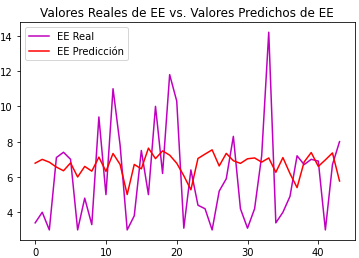
\includegraphics[scale=.7]{F4/F4-im30.PNG}
    \caption{Comparación de los valores de EE vs. los predichos. Modelo Regresión Lineal tercer conjunto de datos.[Creación propia, 2021]}
    \label{fig:EE3.2}
\end{figure}

\begin{figure}[!h]
    \centering
    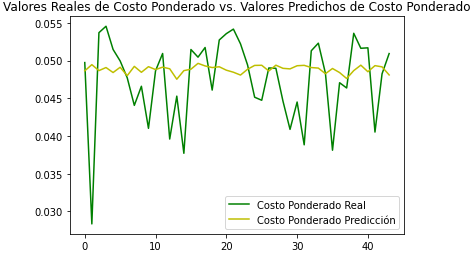
\includegraphics[scale=.7]{F4/F4-im31.PNG}
    \caption{Comparación de los valores de Costo Ponderado vs. los predichos. Modelo Regresión Lineal tercer conjunto de datos.[Creación propia, 2021]}
    \label{fig:CostoPonderado3.2}
\end{figure}

\pagebreak La Figura \ref{fig:EC3.2} sí mantiene el mismo comportamiento de los datos reales pero el resto de las figuras se desvían en gran medida. 

\subsection{Ajustar el modelo evaluando su fiabilidad y su impacto en los objetivos anteriormente establecidos}\label{ajustar}
Utilizando las métricas anteriormente establecidas, evaluamos los modelos.
\subsubsection{Primer conjunto de datos}


Para el conjunto con una cota de 0.075 los resultados son del modelo KNN y la Regresión Lineal se encuentran en las Figuras \ref{fig:MetricasKNN1} y \ref{fig:MetricasMAE1} respectivamente: 


\begin{figure}[!h]
    \centering
    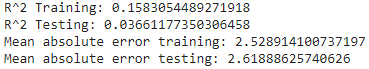
\includegraphics[scale=.7]{F4/F4-im32.PNG}
    \caption{El valor de $R^{2}_{ajustada}$ y el Error Absoluto Medio en modelo KNN primer conjunto. [Creación propia, 2021]}
    \label{fig:MetricasKNN1}
\end{figure}
\begin{figure}[!h]
    \centering
    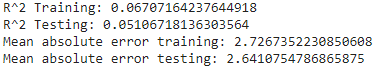
\includegraphics[scale=.7]{F4/F4-im33.PNG}
    \caption{El valor de $R^{2}_{ajustada}$ y el Error Absoluto Medio en modelo Regresión Lineal primer conjunto. [Creación propia, 2021]}
    \label{fig:MetricasMAE1}
\end{figure}
\pagebreak

Una $R^{2}_{ajustada}$ tan pequeña es probablemente resultado de incluir tantos parámetros en la predicción. El Error Absoluto Medio comparado con la dimensión de los datos, está en un rango aceptable. 
\subsubsection{Segundo conjunto de datos}
\begin{figure}[!h]
    \centering
    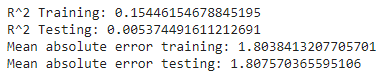
\includegraphics[scale=.7]{F4/F4-im34.PNG}
    \caption{El valor de $R^{2}_{ajustada}$ y el Error Absoluto Medio en modelo KNN segundo conjunto. [Creación propia, 2021]}
    \label{fig:MetricasKNN2}
\end{figure}

\begin{figure}[!h]
    \centering
    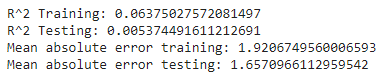
\includegraphics[scale=.7]{F4/F4-im35.PNG}
    \caption{El valor de $R^{2}_{ajustada}$ y el Error Absoluto Medio en modelo Regresión Lineal segundo conjunto. [Creación propia, 2021]}
    \label{fig:MetricasMAE2}
\end{figure}
Los valores del Error Absoluto Medio (Figuras   \ref{fig:MetricasKNN2} y \ref{fig:MetricasMAE2}) disminuyeron, sin embargo la $R^{2}_{ajustada}$ también disminuyó  muy drásticamente. 
\subsubsection{Tercer conjunto de datos}
\begin{figure}[!h]
    \centering
    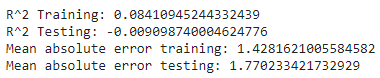
\includegraphics[scale=.7]{F4/F4-im36.PNG}
    \caption{El valor de $R^{2}_{ajustada}$ y el Error Absoluto Medio en modelo KNN tercer conjunto. [Creación propia, 2021]}
    \label{fig:MetricasKNN3}
\end{figure}

\begin{figure}[!h]
    \centering
    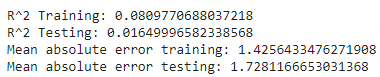
\includegraphics[scale=.7]{F4/F4-im37.PNG}
    \caption{El valor de $R^{2}_{ajustada}$ y el Error Absoluto Medio en modelo Regresión Lineal tercer conjunto. [Creación propia, 2021]}
    \label{fig:MetricasMAE3}
\end{figure}

En estos modelos ambas $R^{2}_{ajustada}$ (Figuras  \ref{fig:MetricasKNN3} y \ref{fig:MetricasMAE3}) son inferiores, en la Figura \ref{fig:MetricasKNN3}
incluso llega a ser negativa. Los Errores Medios Absolutos son semejantes a los del segundo conjunto. 

El modelo de K Nearest Neighbors con K=12 evaluado en el primer conjunto de datos con cota superior de 0.075 es aquel que resulta óptimo pues tiene una $R^{2}_{ajustada}$ más elevada en comparación al resto y su Error Absoluto Medio entra en un rango aceptable tomando en cuenta todos los valores en los modelos. 

\subsubsection{Escalar Variables}

El modelo más óptimo se escalará usando MinMaxScaler (Escalado de Variables), una función que se encarga de escalar las variables de manera que los nuevos valores se encuentren entre el rango dado, en este caso 0 y 1, pero conservando las proporciones. Se utiliza esta función para transformar las variables de entrada. La fórmula (Figura  \ref{fig:EscaladoVariables})  que representa lo que ocurre es:

\begin{figure}[!h]
    \centering
    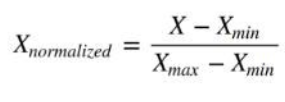
\includegraphics[scale=.7]{F4/F4-im38.PNG}
    \caption{Fórmula de Escalado de Variables.\cite{EscaladoCita1}}
    \label{fig:EscaladoVariables}
\end{figure}

Se eligió este método pues no utiliza ni la desviación estándar ni la media, a diferencia del Escalado Estándar, evitando así cualquier sensibilidad que estás puedan tener. Es importante no utilizar MinMaxScaler cuando los valores son muy estables, sin embargo en este caso nuestras predicciones se caracterizan por sus altas caídas y subidas derivando en que no hay inconveniente al emplear este método.\cite{EscaladoCita1}

Es muy importante al utilizar machine learning escalar, pues hay algoritmos que tienen sensibilidad a los valores mayores, tal es el caso de KNN que, al basarse principalmente en distancias, puede cambiar la percepción de lo que es lejano y cercano al estar escaladas las variables de entrada. \cite{EscaladoCita2}

Escalando los valores de entrada y aplicando el modelo obtenemos (Figura \ref{fig:PrediccionesEscalado} ):
\begin{figure}[!h]
    \centering
    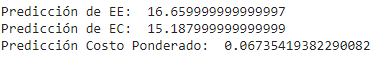
\includegraphics[scale=.7]{F4/F4-im39.PNG}
    \caption{Valores predichos por el modelo escalado.[Creación propia, 2021]}
    \label{fig:PrediccionesEscalado}
\end{figure}
En cuanto a su métrica (Figura \ref{fig:PrediccionesEscalado2}):
\begin{figure}[!h]
    \centering
    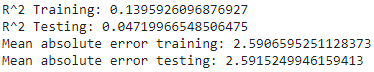
\includegraphics[scale=.7]{F4/F4-im40.PNG}
    \caption{Métricas del modelo escalado.[Creación propia, 2021]}
    \label{fig:PrediccionesEscalado2}
\end{figure}
\pagebreak

Dado a que no hubo un cambio significativo en los valores que predijo el modelo y en cambio hubo un decremento en la $R^{2}_{ajustada}$, por ello se considera que es mejor conservar el modelo original. 

\section{Evaluación}
\subsection{Evaluar el modelo o modelos generados hasta el momento}

Como se menciona en la sección \ref{tecnicas}, el conjunto de datos que mejores resultados entrega es el primero, el cual toma costos ponderados menores o iguales a 0.075. Usando la relación train-test definida en la sección \ref{construir}, se evaluaron los modelos \emph{K nearest neighbors} y  \emph{Multioutput linear regression}. Tras hacer esta evaluación se determinó que el modelo que mejores resultados entrega es \emph{K nearest neighbors}, cuyo parámetro \emph{k} se fijó como 12 (ver figura \ref{fig:Codo1}).


Usando las métricas de Sklearn, podemos evaluar fácilmente este modelo usando $R^{2}_{ajustada}$. Como se mencionó antes, $R^{2}_{ajustada}$ agrega una penalización por cada estimador usado, es por esto que, en nuestro caso, usando 3 estimadores, el valor de $R^{2}_{ajustada}$ sea bajo, esto no necesariamente significa que sea un mal modelo, al contrario, las figuras\ref{fig:EC1.1}, \ref{fig:EE1.1} y \ref{fig:CostoPonderado1.1} nos muestran que, aunque la magnitud no es exacta, el modelo simula de manera correcta el comportamiento de los datos reales, por lo que podemos argumentar que en efecto es un modelo representativo para los datos de esta población. Los resultados de $R^{2}_{ajustada}$ obtenidos son los siguientes:
\begin{figure}[!ht]
    \centering
    \begin{minted}{python}
    R^2 Training: 0.1583054489271918
    R^2 Testing: 0.03661177350306458
    \end{minted}
    \caption{Resultados de $R^2_{ajustada}$ obtenidos con el modelo \emph{K nearest neighbors} con el primer conjunto de datos.[Creación propia, 2021]}
    \label{fig:r2ajtrain}
\end{figure}


 Por su parte, al computar el Error Absoluto Medio obtuvimos lo siguiente:
\begin{figure}
    \centering
    \begin{minted}{python}
    Mean absolute error training: 2.528914100737197
    Mean absolute error testing: 2.61888625740626
    \end{minted}
    \caption{Resultados de \emph{Mean absolute error} obtenidos con el modelo \emph{K nearest neighbors} con el primer conjunto de datos.[Creación propia, 2021]}
    \label{fig:mae}
\end{figure}

Esta métrica es sencilla de comprender pero hay que entender su contexto, estamos hablando de una métrica que nos indica que tanto se equivocan nuestras predicciones, pero no lo hace por separado (es decir por cada variable de salida), por lo que un valor alto podría ser preocupante si se hablara de costo ponderado, pues como se observa en la figura \ref{fig:CostoPonderado1.1}, sus valores son pequeños. Dicho esto, no es el caso, si observamos con atención las figuras \ref{fig:EC1.1}, \ref{fig:EE1.1} y \ref{fig:CostoPonderado1.1} podemos observar que las 3 variables contribuyen de manera más o menos equitativa a este error, es decir, el \emph{MAE} no está siendo sobrecargado por una sola variable con un error muy grande, sino que está distribuido en pequeños errores entre las 3 variables.

Todo lo anterior nos lleva a concluir que en efecto, aunque las métricas obtenidas no son sorprendentes, sin duda se ha logrado un buen modelo, y podemos entender las fuentes de error que se tienen.

\subsection{Revisar todo el proceso de minería de datos que nos ha llevado hasta este punto}
En la sección \ref{objetivos}, se definieron los objetivos de minería de datos del proyecto. Llegada esta etapa podemos decir que se han cumplido con todos los puntos de la Metodología CRISP-DM. No se ha presentado ningún inconveniente para llevar a cabo los métodos y el análisis de los resultados. Se cuenta con un modelo multi entrada y multi salida que entrega resultados satisfactorios y ha sido evaluado con las métricas pertinentes. Además, las correlaciones entre variables fueron comprendidas y evaluadas en la sección \ref{apto}.  

\subsection{Siguientes pasos}

A pesar de que estamos satisfechos con los resultados obtenidos,
hay que recordar que que este es un trabajo de investigación cuya mayor limitante era el tiempo, existen muchos próximos pasos que pueden darse para expandir el alcance de la investigación. A continuación se muestran 2 propuestas que darían una buena continuidad a este proyecto.

\subsubsection{Conectar el modelo a un ecosistema MapReduce en Hadoop para obtener datos de entornos de producción en tiempo real}

Una vez que se ha consolidado un modelo funcional que cumple con las expectativas del cliente, se puede conectar a un entorno de Hadoop data streaming \cite{hadoop}, de esta manera se pueden procesar cantidades enormes de información de una manera eficiente, sencilla, escalable y barata (gracias a las ventajas que ofrece la computación en la nube). Conforme se tengan más datos disponibles, se comprenderá de una mejor manera como se comportan y de esta manera se conseguirá un modelo que irá mejorando con el tiempo, y que eventualmente cumplirá la función de optimizar los costos de la mejor manera posible, sin reducir la calidad. 

\subsubsection{Usar Hyperparameter Tuning para obtener el modelo más óptimo posible, para su posterior implementación en producción}

Si bien es cierto que se ha obtenido un buen modelo, y que la intervención humana puede ayudar a crear buenos modelos, la realidad es que hay límites en cuanto a el número de modelos que podemos probar. Es por eso que usar la técnica conocida como Hyperparameter tuning suena como una muy buena opción.

La documentación de Amazon Web Services menciona la búsqueda Bayesiana, esta funciona como una regresión. Consiste en optimizar un modelo para la métrica de nuestra elección adivinando que combinaciones de parametros son mas propensas a brindar mejores resultados, para posteriormente correr tareas de entrenamiento y prueba, para verificar los resultados obtenidos. \cite{hyperpar}

Esta técnica no requiere muchos recursos, basta con crear una instancia de \emph{AWS Sage maker} para correr la optimización Bayesiana. Aunque es posible que esta tarde un tiempo considerable en encontrar los parámetros óptimos, considerando que las instancias de sage maker son económicas pues se cobran bajo el modelo \emph{Paga por lo que usas}, la realidad es que valdrá la pena la inversión, sobre todo por que solo se pagaría por cada vez que se desee correr esta optimización. 

\section{Conclusión general del equipo}

Dada la naturaleza de los datos y la cantidad de parámetros, es normal que el modelo no sea completamente exacto, sin embargo lo esencial es que sigue el mismo comportamiento que los datos originales, por ello podemos concluir que es un modelo funcional para optimizar el gasto de la energía eléctrica y el gasto de la energía combustible. Aumentar la $R^2_ajustada$ o disminuir el Error Absoluto Medio,  lo convertiría en un modelo ideal sin embargo es posible que sea necesario recabar más datos o utilizar menos parámetros pero tengan una correlación más alta con las variables de salida para lograrlo.
\section{Aportaciones Individuales}
A01246619 Salette Noemi
\begin{itemize}
\item Análisis de Correlación entre las variables
\item Costo, Costo Ponderado, EE Ponderado, EC Ponderado
\item Método Kneighbours y multiple linear regression
\item Gráficas de predicciones contra valores reales
\item Evaluación de modelos
\item Primer Grupo de Valores (sección)
\item Segundo Grupo de Valores (sección)
\item Tercer Grupo de Valores (sección)
\end{itemize}

A01620402 Miguel Chávez
\begin{itemize}
\item Importación de datos y cambio de índice de fecha
\item Dispersiones de energía eléctrica y combustible respecto a tasa de producción
\item Limpieza de datos atípicos y nulos
\item Matriz de correlaciones
\item Separación de training set y test set
\end{itemize}
A01174385 Francisco Leonid Gálvez Flores
\begin{itemize}
\item Gráfica 3D
\item Decision Tree (descartado)
\item Support Vector Machine (Regressor) (descartado)
\end{itemize}
A00828359 Isaac Arredondo Padrón
\begin{itemize}
    \item Gráficas Pairplot
\end{itemize}

\section{Bibliografía}
\bibliographystyle{apalike}

\bibliography{fuentes.bib}


\end{document}
